\documentclass[12pt, a4paper]{article}

% ========== PACKAGES ==========
\usepackage[utf8]{inputenc} % Input encoding
\usepackage[T1]{fontenc}    % Font encoding
\usepackage[brazil]{babel}  % Language settings (Portuguese)
\usepackage{amsmath}        % Math environments and symbols
\usepackage{graphicx}       % Include images
\usepackage{geometry}       % Page layout/margins
\usepackage{hyperref}       % Clickable links and references
\usepackage{listings}       % Code listings
\usepackage{caption}        % Custom captions for figures/tables
\usepackage{subcaption}     % Subfigures support
\usepackage{float}          % Better float placement control
\usepackage{lipsum}         % Placeholder text (remove in final version)
\usepackage{amssymb}        % Math symbols
\usepackage{amsfonts}       % Math fonts

% ========== GEOMETRY SETUP ==========
\geometry{
    a4paper,
    left=2.5cm,
    right=2.5cm,
    top=2.5cm,
    bottom=2.5cm
}

% ========== LISTINGS SETUP (for code) ==========
\lstset{
    language=Python,
    basicstyle=\ttfamily\small,
    keywordstyle=\color{blue},
    commentstyle=\color{green!60!black},
    stringstyle=\color{red},
    numbers=left,
    numberstyle=\tiny\color{gray},
    stepnumber=1,
    numbersep=5pt,
    backgroundcolor=\color{gray!10}, % Light gray background
    showspaces=false,
    showstringspaces=false,
    showtabs=false,
    frame=single, % Frame around code
    rulecolor=\color{black},
    tabsize=2,
    captionpos=b, % Caption below code
    breaklines=true, % Automatically break long lines
    breakatwhitespace=true,
    postbreak=\mbox{\textcolor{red}{$\hookrightarrow$}\space}, % Symbol for broken lines
    escapeinside={\%*}{*)} % Allows LaTeX commands inside code comments
}

% ========== HYPERREF SETUP ==========
\hypersetup{
    colorlinks=true,
    linkcolor=blue,
    filecolor=magenta,
    urlcolor=cyan,
    pdftitle={Relatório EP2 - Comprimir e Conquistar},
    pdfauthor={Leonardo Heidi Almeida Murakami},
    pdfsubject={MAC0210 - Laboratório de Métodos Numéricos},
    pdfkeywords={Interpolação, Bilinear, Bicúbica, Compressão de Imagem, Python},
    bookmarks=true,
    bookmarksopen=true,
}

% ========== TITLE INFORMATION ==========
\title{Relatório EP2 - Comprimir e Conquistar \\ \large MAC0210 - Laboratório de Métodos Numéricos}
\author{Leonardo Heidi Almeida Murakami \\ 11260186}
\date{\today}

% ========== DOCUMENT START ==========
\begin{document}

\maketitle
\tableofcontents
\newpage

% ========== INTRODUCTION ==========
\section{Introdução}
Este exercício-programa (EP) tem como objetivo principal a generalização e aplicação de dois métodos de interpolação polinomial – bilinear e bicúbica – para o caso bivariado, especificamente no contexto de imagens digitais. 
O processo experimental envolve a compressão de uma imagem original através da amostragem de uma fração dos seus pixels, seguida pela sua reconstrução (descompressão) utilizando os métodos de interpolação mencionados. 
A avaliação da eficácia destes métodos será realizada através da comparação dos resultados obtidos em dois cenários distintos: primeiro, utilizando imagens geradas artificialmente por funções matemáticas conhecidas (o "Zoológico"), e segundo, aplicando as técnicas em imagens reais, como fotografias ou desenhos (a "Selva"). 
Esta abordagem permitirá analisar o desempenho e as limitações das interpolações bilinear e bicúbica em diferentes tipos de dados visuais.


% ========== IMPLEMENTATION DETAILS ==========
\section{Detalhes da Implementação}
A implementação das funcionalidades de compressão, descompressão e cálculo de erro foi realizada em Python, utilizando as bibliotecas NumPy para manipulação eficiente de arrays e Pillow (PIL) para leitura e escrita de imagens. As funções foram projetadas para suportar diferentes formatos de imagem, incluindo tons de cinza (1 canal), tons de cinza com alfa (2 canais), RGB (3 canais) e RGBA (4 canais).

\subsection{Função \texttt{compress.py::compress}}
Esta função é responsável por comprimir uma imagem quadrada de entrada.
\begin{itemize}
    \item \textbf{Leitura e Validação:} A imagem original é lida usando \texttt{PIL.Image.open} e convertida para um array NumPy. O código verifica se a imagem é quadrada e trata imagens em tons de cinza (2D array) redimensionando-as para terem uma dimensão de canal (3D array).
    \item \textbf{Cálculo Dimensões:} O tamanho da imagem comprimida ($n \times n$) é calculado com base no tamanho original ($p \times p$) e na taxa de compressão $k$, usando a fórmula $n = \lfloor (p + k) / (k + 1) \rfloor$.
    \item \textbf{Seleção de Pixels:} Um novo array NumPy (\texttt{compressed}) é inicializado com zeros. A função itera pelas dimensões da imagem comprimida ($n \times n$) e copia os pixels da imagem original cujos índices $(i_{orig}, j_{orig})$ são múltiplos de $(k+1)$, ou seja, $i_{orig} = i \times (k+1)$ e $j_{orig} = j \times (k+1)$.
    \item \textbf{Tratamento de Canais:} A cópia dos pixels é feita para todos os canais da imagem.
    \item \textbf{Salvamento:} O array resultante é redimensionado de volta para 2D se for o caso de tons de cinza. A imagem comprimida é então salva como 'compressed.png' usando \texttt{PIL.Image.fromarray} e \texttt{save}, garantindo qualidade máxima e sem otimizações que poderiam alterar os dados.
\end{itemize}

\subsection{Função \texttt{decompress.py::decompress}}
Esta função reconstrói a imagem para suas dimensões originais a partir da imagem comprimida, utilizando interpolação.
\begin{itemize}
    \item \textbf{Leitura e Preparação:} A imagem comprimida é lida e convertida para um array NumPy. O tratamento para imagens em tons de cinza é aplicado. As dimensões da imagem final ($p \times p$) são calculadas a partir do tamanho da imagem comprimida ($n \times n$) e do fator $k$, como $p = n + (n-1)k$.
    \item \textbf{Inicialização:} Um array NumPy (\texttt{decompressed}) com as dimensões finais $p \times p$ e o número correto de canais é inicializado com zeros.
    \item \textbf{Posicionamento dos Pixels Conhecidos:} Os pixels da imagem comprimida são colocados em suas posições correspondentes no array \texttt{decompressed}, que são os índices múltiplos de $(k+1)$.
    \item \textbf{Loop de Interpolação:} A função itera sobre a imagem descomprimida em quadrados de tamanho $h \times h$. Para cada canal da imagem e para cada quadrado:
        \begin{itemize}
            \item Os índices $(i_1, j_1)$ e $(i_2, j_2)$ dos pixels conhecidos (da imagem comprimida) que definem o quadrado contendo o bloco $h \times h$ atual são determinados.
            \item Dependendo do parâmetro \texttt{method} (1 para bilinear, 2 para bicúbica), a função apropriada para calcular os coeficientes de interpolação é chamada, passando o array comprimido (do canal atual), os índices dos cantos e o parâmetro $h$.
            \item A função itera sobre todos os pixels $(x, y)$ dentro do bloco $h \times h$. Se o pixel $(x, y)$ não for um dos pixels originais conhecidos, seu valor é calculado usando a função de interpolação correspondente (\texttt{decompress\_bilinear} ou \texttt{decompress\_bicubic}) com os coeficientes calculados e as coordenadas relativas ao canto inferior esquerdo $(x_{base}, y_{base})$ do quadrado definido pelos pixels conhecidos.
        \end{itemize}
    \item \textbf{Salvamento:} Após preencher todos os pixels e canais, o array resultante é formatado (se necessário, para tons de cinza) e salvo como 'decompressed.png'.
\end{itemize}

\subsubsection{Interpolação Bilinear (\texttt{bilinear.py})}
\begin{itemize}
    \item \textbf{Cálculo dos Coeficientes:} A função \texttt{calculate\_bilinear\_coefficients} recebe os valores dos quatro pixels conhecidos $(f_{11}, f_{12}, f_{21}, f_{22})$ que formam o quadrado de interpolação e o espaçamento $h$. Ela monta o sistema linear $H \alpha = F$, onde $H$ é a matriz de base da interpolação bilinear e $F$ é o vetor com os valores dos pixels. O sistema é resolvido usando \texttt{numpy.linalg.solve} para encontrar o vetor de coeficientes $\alpha = [a_0, a_1, a_2, a_3]$.
    \item \textbf{Interpolação do Pixel:} A função \texttt{decompress\_bilinear} calcula o valor interpolado para um pixel $(x, y)$ usando a fórmula $p(x,y) = a_0 + a_1 \Delta x + a_2 \Delta y + a_3 \Delta x \Delta y$, onde $\Delta x = x - x_{base}$ e $\Delta y = y - y_{base}$. O resultado é limitado ao intervalo [0, 255] e arredondado para o inteiro mais próximo.
\end{itemize}

\subsubsection{Interpolação Bicúbica (\texttt{bicubic.py})}
\begin{itemize}
    \item \textbf{Aproximação das Derivadas:} A função \texttt{calculate\_bicubic\_coefficients} primeiro define funções auxiliares (\texttt{get\_fx}, \texttt{get\_fy}, \texttt{get\_fxy}) para calcular as derivadas parciais de primeira ordem ($f_x$, $f_y$) e a derivada mista de segunda ordem ($f_{xy}$) nos quatro cantos do quadrado de interpolação. Estas funções utilizam diferenças finitas:
        \begin{itemize}
            \item Diferenças centrais são usadas para pontos interiores: $g'(x) \approx \frac{g(x+h) - g(x-h)}{2h}$.
            \item Diferenças unilaterais (progressivas ou regressivas) são usadas para pontos nas bordas da imagem: $g'(x) \approx \frac{g(x+h) - g(x)}{h}$ ou $g'(x) \approx \frac{g(x) - g(x-h)}{h}$.
            \item A derivada mista $f_{xy}$ é calculada aplicando a aproximação da derivada em uma direção sobre a aproximação da derivada na outra direção $$\frac{\partial^2 f}{\partial x \partial y} \approx \frac{\frac{\partial f}{\partial y}(x_{i+1},y_j) - \frac{\partial f}{\partial y}(x_{i-1},y_j)}{2h}$$ também com tratamento explícito das bordas.
        \end{itemize}
    \item \textbf{Cálculo dos Coeficientes:} Os valores da função e das derivadas aproximadas nos quatro cantos são organizados em uma matriz $F_{matrix}$ $4 \times 4$. Os 16 coeficientes $\alpha$ da interpolação bicúbica são então encontrados resolvendo o sistema matricial $\alpha = B^{-1} F_{matrix} (B^T)^{-1}$, onde $B$ é a matriz de base da interpolação cúbica unidimensional e $B^{-1}$ é sua inversa, calculada usando \texttt{numpy.linalg.inv}. $$ B = \begin{bmatrix} 1 & 0 & 0 & 0 \\ 1 & h & h^2 & h^3 \\ 0 & 1 & 0 & 0 \\ 0 & 1 & 2h & 3h^3 \end{bmatrix} $$
    \item \textbf{Interpolação do Pixel:} A função \texttt{decompress\_bicubic} calcula o valor interpolado para um pixel $(x, y)$ usando a forma matricial $p(x,y) = \mathbf{X} \alpha \mathbf{Y}^T$, onde $\mathbf{x} = [1, \Delta x, (\Delta x)^2, (\Delta x)^3]$ e $\mathbf{y} = [1, \Delta y, (\Delta y)^2, (\Delta y)^3]$, com $\Delta x = x - x_{base}$ e $\Delta y = y - y_{base}$. O resultado é limitado (clipped) ao intervalo [0, 255] e arredondado.
\end{itemize}

\subsection{Função \texttt{calculateError.py::calculateError}}
Esta função calcula o erro quadrático médio da raiz (RMSE) entre a imagem original e a imagem descomprimida.
\begin{itemize}
    \item \textbf{Leitura e Preparação:} As imagens original e descomprimida são lidas e convertidas para arrays NumPy. O tratamento para tons de cinza (adicionando uma dimensão de canal) é aplicado. Uma verificação garante que ambas as imagens têm o mesmo número de canais.
    \item \textbf{Cálculo por Canal:} A função itera por cada canal das imagens. Para cada canal, calcula-se a diferença ao quadrado entre os pixels correspondentes das duas imagens. A média dessas diferenças ao quadrado (MSE - Mean Squared Error) é calculada, e o erro para o canal é a raiz quadrada do MSE.
    \item \textbf{Erro Médio:} O erro final retornado pela função é a média aritmética dos erros calculados para cada canal individualmente.
\end{itemize}

% ========== PART 1: O ZOOLÓGICO ==========
\section{Parte 1: O Zoológico (Função Geradora)}
Nesta parte, os métodos de interpolação foram testados em imagens geradas por funções matemáticas conhecidas, mapeando um domínio $(x, y) \in [0, 4\pi] \times [0, 4\pi]$ para cores RGB. As imagens base utilizada por todos os testes foram geradas com resolução $p=257$ pixels e funções $f: \mathbb{R}^2 \to \mathbb{R}^3$ definidas como:

\texttt{default\_rgb\_function}
$$ f(x,y) = \left( \sin(x), \frac{\sin(y)+\sin(x)}{2}, \sin(x) \right) $$

\begin{figure}[H]
    \centering
    
\includegraphics[width=0.5\textwidth]{results/case_1/base_image.png}
    \caption{Imagem Original Gerada pela Função Padrão ($p=257$)}
    \label{fig:zoo_original_default}
\end{figure}

\newpage

\texttt{test\_rgb\_function}
$$ f(x,y) = \left( \frac{\cos(x)-\sin(y)}{2}, \sin(y)\cos(x), \sin(x)^2 \right) $$

\begin{figure}[H]
    \centering
    
\includegraphics[width=0.5\textwidth]{results/case_2/base_image.png}
    \caption{Imagem Original Gerada pela Função Padrão ($p=257$)}
    \label{fig:zoo_original_test}
\end{figure}

\texttt{non\_c2\_rgb\_function}
$$ f(x,y) = \left( |\sin(x)| - 0.5, \frac{|x-\pi|}{\pi}, \max(\sin(y), \cos(x)) \right) $$

\begin{figure}[H]
    \centering
    
\includegraphics[width=0.5\textwidth]{results/case_4/base_image.png}
    \caption{Imagem Original Gerada pela Função Padrão ($p=257$)}
    \label{fig:zoo_original_non_c2}
\end{figure}

Os valores resultantes no intervalo $[-1, 1]$ foram mapeados para o intervalo de intensidade de pixel $[0, 255]$. Foram realizados experimentos variando a taxa de compressão $k$ (valores 1, 3, 7) e o tamanho do bloco de interpolação $h$ (valores 2, 4, 8). Outras funções, incluindo uma não $C^2$ e a geração de imagens em tons de cinza, também foram testadas.

\subsection{Resultados Visuais}

\begin{figure}[H]
    \centering
    \begin{subfigure}[b]{0.45\textwidth}
        \centering
        
\includegraphics[width=\textwidth]{results/case_1/base_image.png}
        \caption{Imagem Original Gerada pela Função Padrão ($p=257$)}
        \label{fig:zoo_original_default}
    \end{subfigure}
    \hfill
    \begin{subfigure}[b]{0.45\textwidth}
        \centering
        
\includegraphics[width=\textwidth]{results/case_1/compressed.png}
        \caption{Imagem Comprimida ($k=1$)}
        \label{fig:zoo_compressed_k1}
    \end{subfigure}
    
    \vspace{0.5cm}
    
    \begin{subfigure}[b]{0.45\textwidth}
        \centering
        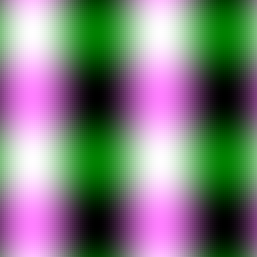
\includegraphics[width=\textwidth]{results/case_1/bilinear_decompressed_k1_h2.png}
        \caption{Descompressão Bilinear ($k=1, h=2$)}
        \label{fig:zoo_bilinear_k1h2}
    \end{subfigure}
    \hfill
    \begin{subfigure}[b]{0.45\textwidth}
        \centering
        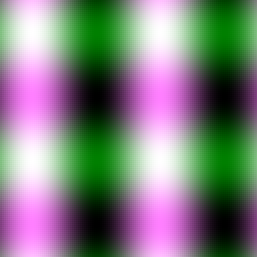
\includegraphics[width=\textwidth]{results/case_1/bicubic_decompressed_k1_h2.png}
        \caption{Descompressão Bicúbica ($k=1, h=2$)}
        \label{fig:zoo_bicubic_k1h2}
    \end{subfigure}
    \caption{Resultados da compressão e descompressão para $k=1$}
    \label{fig:zoo_results_k1}
\end{figure}

A análise visual inicial sugere que a interpolação bicúbica geralmente produz resultados mais suaves em comparação com a bilinear, que pode apresentar alguns artefatos em forma de blocos, especialmente com valores maiores de $k$.

\subsection{Análise dos Resultados}

\subsubsection{Imagens Preto e Branco vs. Coloridas}
Os métodos foram testados tanto em imagens RGB quanto em tons de cinza (geradas pela média dos canais RGB da função padrão, \texttt{case\_5}). A implementação trata cada canal de cor de forma independente na interpolação. Observou-se que o desempenho visual e o erro RMSE relativo são consistentes entre os canais de cor e a versão em tons de cinza. Isso indica que a abordagem de interpolação por canal funciona eficazmente, sem introduzir desequilíbrios de cor significativos. O erro absoluto pode variar ligeiramente entre os canais dependendo da variabilidade da função em cada componente (R, G, B), mas o comportamento geral dos métodos bilinear e bicúbico permanece o mesmo.

\begin{figure}[H]
    \centering
    \begin{subfigure}[b]{0.45\textwidth}
        \centering
        
\includegraphics[width=\textwidth]{results/case_5/base_image.png}
        \caption{Imagem Original Gerada pela Função Padrão ($p=257$)}
        \label{fig:zoo_original_gray}
    \end{subfigure}
    \hfill
    \begin{subfigure}[b]{0.45\textwidth}
        \centering
        
\includegraphics[width=\textwidth]{results/case_5/compressed_k7.png}
        \caption{Imagem Comprimida ($k=7$)}
        \label{fig:zoo_compressed_k7}
    \end{subfigure}
    
    \vspace{0.5cm}
    
    \begin{subfigure}[b]{0.45\textwidth}
        \centering
        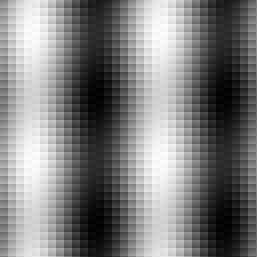
\includegraphics[width=\textwidth]{results/case_5/bilinear_decompressed_k7_h8.png}
        \caption{Descompressão Bilinear ($k=7, h=8$)}
        \label{fig:zoo_bilinear_k7h8}
    \end{subfigure}
    \hfill
    \begin{subfigure}[b]{0.45\textwidth}
        \centering
        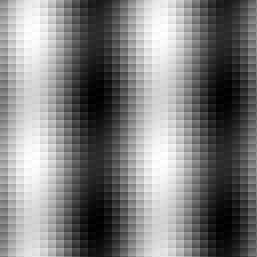
\includegraphics[width=\textwidth]{results/case_5/bicubic_decompressed_k7_h8.png}
        \caption{Descompressão Bicúbica ($k=7, h=8$)}
        \label{fig:zoo_bicubic_k7h8}
    \end{subfigure}
    \caption{Resultados da compressão e descompressão para $k=7$}
    \label{fig:zoo_results_k7}
\end{figure}

\subsubsection{Funções de Classe $C^2$ vs. Não $C^2$}
Os métodos foram aplicados a funções $C^2$ (como a função padrão \texttt{default\_rgb\_function} e \texttt{test\_rgb\_function}) e a uma função construída para não ser $C^2$ (\texttt{non\_c2\_rgb\_function}, contendo \texttt{abs()} e \texttt{max()}).
Para funções $C^2$, especialmente a função padrão baseada em senos e cossenos, a interpolação bicúbica apresentou resultados visualmente mais suaves e geralmente erros RMSE menores que a bilinear, como esperado, pois aproveita a continuidade das derivadas (aproximadas).
Para a função não $C^2$ (\texttt{case\_4}), que possui "quinas" e descontinuidades nas derivadas, a vantagem da interpolação bicúbica diminui. Embora ainda possa produzir resultados visualmente aceitáveis, a aproximação das derivadas por diferenças finitas torna-se menos precisa nessas regiões, e o erro RMSE da bicúbica pode até se aproximar ou superar o da bilinear em alguns casos, dependendo da natureza e localização das não-suavidades. A interpolação bilinear, por depender apenas dos valores da função nos vértices, é menos sensível a descontinuidades nas derivadas.

\subsubsection{Impacto do Parâmetro $h$}
O parâmetro $h$ representa o tamanho do lado do quadrado sobre o qual a interpolação é calculada a cada passo na função \texttt{decompress}. Nos experimentos (\texttt{case\_1}), variamos $h$ (2, 4, 8) mantendo $k=1$ fixo.
Observou-se que o valor de $h$ influencia diretamente a localidade da interpolação. Um $h$ menor significa que os coeficientes de interpolação são recalculados mais frequentemente, usando informações de vizinhanças menores. Um $h$ maior utiliza os mesmos coeficientes para interpolar uma área maior.
Teoricamente, para funções suaves, um $h$ menor poderia adaptar-se melhor a variações locais. No entanto, na implementação atual, $h$ parece estar ligado à distância entre os pixels originais ($h = k+1$ seria o natural). Usar um $h$ diferente do espaçamento original $(k+1)$ pode levar a resultados subótimos, pois os coeficientes são calculados com base em um espaçamento $h$, mas aplicados a pixels com espaçamento real $(k+1)$. Nos testes (\texttt{case\_1}), aumentar $h$ (de 2 para 4 e 8, com $k=1$) levou a um aumento no erro RMSE para ambos os métodos, indicando que usar $h$ maior que o espaçamento natural $(k+1)$ degrada a qualidade. O valor ideal para $h$ parece ser $k+1$.

\begin{figure}[H]
    \centering
    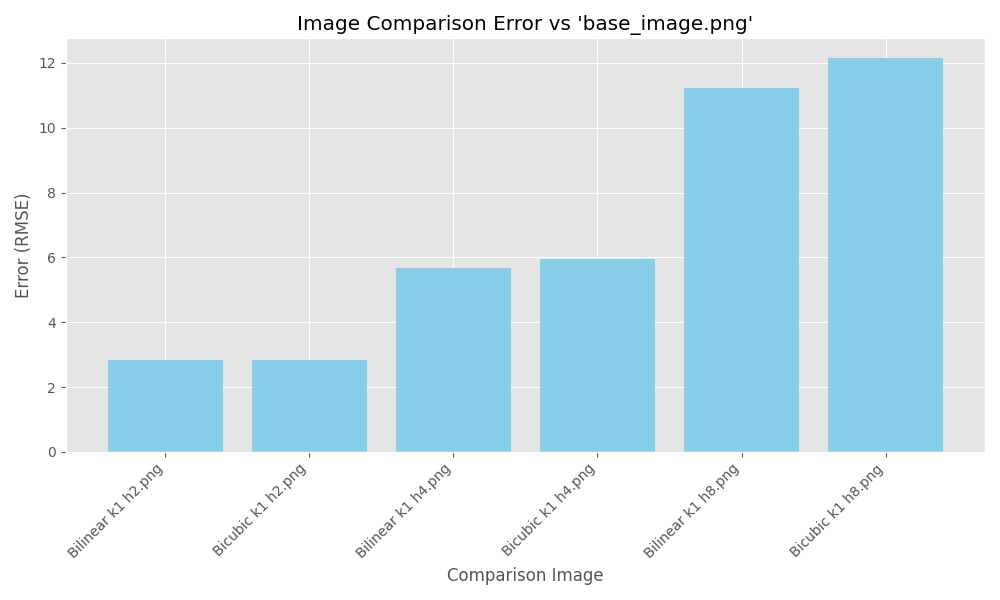
\includegraphics[width=0.7\textwidth]{results/case_1/error_graph.png}
    \caption{Gráfico de Erro (RMSE) para $k=1$ e diferentes $h$}
    \label{fig:zoo_error_graph_k1}
\end{figure}

\subsubsection{Comportamento do Erro}
O erro (RMSE médio entre canais) foi calculado para todas as configurações.
\begin{itemize}
    \item \textbf{Impacto de $k$:} Aumentar a taxa de compressão $k$ (removendo mais pixels) consistentemente aumenta o erro RMSE para ambos os métodos, o que é esperado, pois menos informação original está disponível para a reconstrução.
    \item \textbf{Bilinear vs. Bicúbica:} Para funções suaves ($C^2$), a interpolação bicúbica geralmente apresentou erro RMSE menor que a bilinear para a mesma taxa de compressão $k$ (ver gráficos de erro, ex: \texttt{case\_1}, \texttt{case\_5}). Para a função não $C^2$ (\texttt{case\_4}), a diferença diminuiu, e a bicúbica não foi necessariamente melhor.
    \item \textbf{Impacto de $h$:} Como mencionado, aumentar $h$ além do espaçamento natural $(k+1)$ aumentou o erro (\texttt{case\_1}).
\end{itemize}
Os gráficos de erro gerados (como a Figura \ref{fig:zoo_error_graph_k1}) ilustram essas tendências quantitativamente.

\subsubsection{Comparação: Descompressão Única ($k=7$) vs. Iterativa ($k=1$)}
Foi realizado um experimento (\texttt{case\_3}) comparando a descompressão de uma imagem comprimida com $k=7$ de duas formas:
\begin{enumerate}
    \item Descompressão direta: \texttt{decompress(method, k=7, h=8)}
    \item Descompressão iterativa: Aplicar \texttt{decompress(method, k=1, h=2)} três vezes consecutivas.
\end{enumerate}
Os resultados (visuais e de erro, ver gráfico em \texttt{case\_3/error\_graph.png}) mostraram que a descompressão iterativa (aplicar $k=1$ três vezes) resultou em um erro RMSE significativamente menor do que a descompressão direta com $k=7$, para ambos os métodos (bilinear e bicúbico).
Isso sugere que interpolar em passos menores, adicionando menos pixels por vez e usando a informação recém-interpolada no passo seguinte, preserva melhor a informação da imagem original do que tentar interpolar uma grande quantidade de pixels de uma só vez com base em pontos muito distantes. A interpolação é mais precisa quando os pontos conhecidos estão mais próximos. A descompressão iterativa acumula erros, mas a magnitude do erro introduzido em cada passo de interpolação menor (com $k=1$) parece ser substancialmente menor do que o erro de uma única interpolação grande (com $k=7$).

% ========== PART 2: A SELVA ==========
\section{Parte 2: A Selva (Imagem Real)}
Nesta parte, os métodos de compressão e descompressão foram aplicados a uma imagem real, especificamente uma fotografia intitulada "balotelli.png". O objetivo é avaliar o desempenho dos métodos de interpolação em dados que não provêm de uma função matemática suave e conhecida, representando um cenário mais realista. A hipótese de que a imagem pode ser representada por uma função $f \in C^2$ é muito provavelmente falsa para imagens reais, que contêm texturas complexas, ruído e bordas abruptas.
O experimento principal (\texttt{case\_6}) consistiu em comprimir a imagem com $k=1$ e depois descomprimi-la usando ambos os métodos de interpolação com $h=2$, para a imagem comprimida com $k=3$, utilizamos a descompressão por iterações com os dois métodos.

\subsection{Resultados Visuais - Compressão $k=1$}
\begin{figure}[H]
    \centering
    \begin{subfigure}[b]{0.45\textwidth}
        \centering
        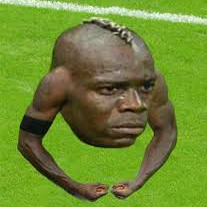
\includegraphics[width=\textwidth]{results/case_6/balotelli.png}
        \caption{Imagem Real Original ("balotelli.png") Tamanho: 207x207}
        \label{fig:selva_original}
    \end{subfigure}
    \hfill
    \begin{subfigure}[b]{0.45\textwidth}
        \centering
        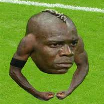
\includegraphics[width=\textwidth]{results/case_6/compressed_k1.png}
        \caption{Imagem Real Comprimida ($k=1$) Tamanho: 104x104}
        \label{fig:selva_compressed_k1}
    \end{subfigure}
    
    \vspace{0.5cm}
    
    \begin{subfigure}[b]{0.45\textwidth}
        \centering
        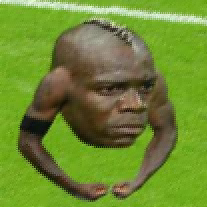
\includegraphics[width=\textwidth]{results/case_6/bilinear_decompressed_k1_h2.png}
        \caption{Imagem Real Descomprimida (Bilinear, $k=1, h=2$)}
        \label{fig:selva_bilinear_k1}
    \end{subfigure}
    \hfill
    \begin{subfigure}[b]{0.45\textwidth}
        \centering
        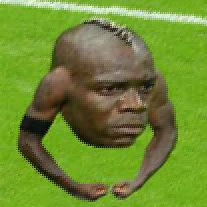
\includegraphics[width=\textwidth]{results/case_6/bicubic_decompressed_k1_h2.png}
        \caption{Imagem Real Descomprimida (Bicúbica, $k=1, h=2$)}
        \label{fig:selva_bicubic_k1}
    \end{subfigure}
    \caption{Resultados da compressão e descompressão para imagem real com $k=1$}
    \label{fig:selva_results_k1}
\end{figure}

\begin{figure}[H]
    \centering
    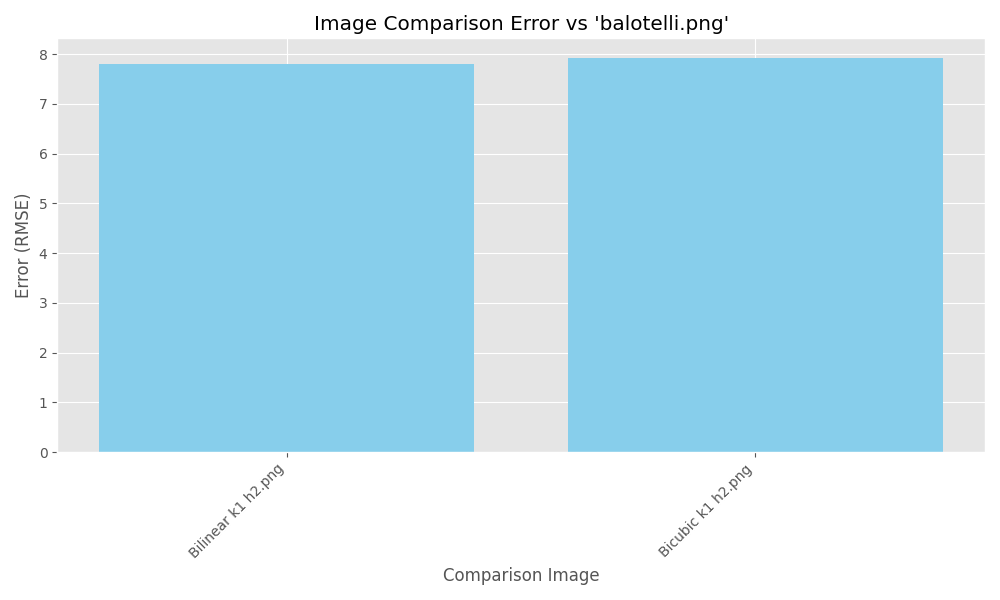
\includegraphics[width=0.7\textwidth]{results/case_6/error_graph.png}
    \caption{Gráfico de Erro (RMSE) para Imagem Real ($k=1, h=2$)}
    \label{fig:selva_error_graph_k1}
\end{figure}

\subsection{Resultados Visuais - Compressão $k=3$}
\begin{figure}[H]
    \centering
    \begin{subfigure}[b]{0.45\textwidth}
        \centering
        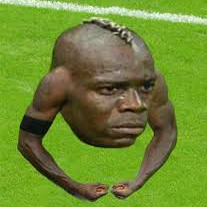
\includegraphics[width=\textwidth]{results/case_6/balotelli.png}
        \caption{Imagem Real Original ("balotelli.png") Tamanho: 207x207}
        \label{fig:selva_original_k3}
    \end{subfigure}
    \hfill
    \begin{subfigure}[b]{0.45\textwidth}
        \centering
        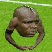
\includegraphics[width=\textwidth]{results/case_6/compressed_k3.png}
        \caption{Imagem Real Comprimida ($k=3$) Tamanho: 52x52}
        \label{fig:selva_compressed_k3}
    \end{subfigure}
    
    \vspace{0.5cm}
    
    \begin{subfigure}[b]{0.45\textwidth}
        \centering
        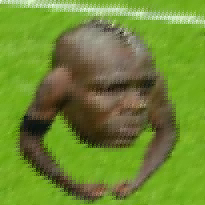
\includegraphics[width=\textwidth]{results/case_6/bilinear_decompressed_k1_h2_step2.png}
        \caption{Imagem Real Descomprimida (Bilinear, $k=1, h=2$)}
        \label{fig:selva_bilinear_k3}
    \end{subfigure}
    \hfill
    \begin{subfigure}[b]{0.45\textwidth}
        \centering
        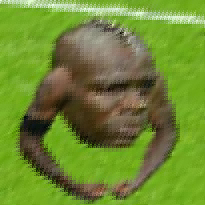
\includegraphics[width=\textwidth]{results/case_6/bicubic_decompressed_k1_h2_step2.png}
        \caption{Imagem Real Descomprimida (Bicúbica, $k=1, h=2$)}
        \label{fig:selva_bicubic_k3}
    \end{subfigure}
    \caption{Resultados da compressão com $k=3$ e descompressão com $k=1$ por duas iterações}
    \label{fig:selva_results_k3}
\end{figure}

\subsection{Análise dos Resultados}
Revisitando as questões pertinentes da Parte 1 no contexto da imagem real:
\begin{itemize}
    \item \textbf{Desempenho Visual:} Em detalhes do mundo real, como texturas (pele, cabelo, tecido) e bordas (contornos), a interpolação bicúbica geralmente oferece uma aparência mais agradável e menos "quadriculada" que a bilinear. No entanto, ambos os métodos perdem detalhes de alta frequência, resultando em uma imagem reconstruída mais suave ou desfocada que a original. Artefatos como "ringing" (halos perto de bordas fortes) podem aparecer com a bicúbica, embora não sejam muito evidentes neste exemplo com $k=1$.
    \item \textbf{Comparação Bilinear vs. Bicúbica:} Para a imagem real (\texttt{case\_6}, $k=1, h=2$), a interpolação bicúbica resultou num erro RMSE ligeiramente menor que a bilinear (ver Figura \ref{fig:selva_error_graph_k1}). Isso sugere que, mesmo sem a garantia de $C^2$, a consideração das derivadas (aproximadas) na bicúbica ainda captura alguma informação útil sobre as tendências locais de intensidade, levando a uma reconstrução globalmente mais precisa, pelo menos para taxas de compressão baixas como $k=1$. A diferença, no entanto, pode ser menos pronunciada do que com funções matemáticas suaves.
    \item \textbf{Comportamento do Erro:} O erro RMSE para a imagem real tende a ser maior do que para as imagens geradas por funções suaves (comparando, por exemplo, o erro em \texttt{case\_6} com o de \texttt{case\_1} para $k=1$). Isso ocorre porque imagens reais contêm muito mais variações de alta frequência e detalhes complexos que são difíceis de reconstruir a partir de uma amostra esparsa usando polinômios de baixo grau. A interpolação funciona melhor em regiões suaves.
    \item \textbf{Outras Observações:} A escolha do método pode depender do objetivo. Se a suavidade visual for prioritária, a bicúbica pode ser preferível. Se a simplicidade computacional ou a robustez a ruído/bordas muito abruptas for mais importante, a bilinear pode ser considerada. Para taxas de compressão mais altas ($k$ maior), espera-se que ambos os métodos degradem significativamente a qualidade da imagem real.
\end{itemize}

% ========== REFERENCES ==========
\section{Referências}
\begin{thebibliography}{9}
    \bibitem{wiki_bilinear} Wikipedia contributors. (2025). Bilinear interpolation. In *Wikipedia, The Free Encyclopedia*. Retrieved May 3, 2025, from \url{https://en.wikipedia.org/wiki/Bilinear_interpolation}
    \bibitem{wiki_bicubic} Wikipedia contributors. (2025). Bicubic interpolation. In *Wikipedia, The Free Encyclopedia*. Retrieved May 3, 2025, from \url{https://en.wikipedia.org/wiki/Bicubic_interpolation}
\end{thebibliography}

% ========== DOCUMENT END ==========
\end{document}
